%*******************************************************************************
% Title: A botnet showcase
%
% Series: Courseworks in Computer Security
%
% Author: Giacomo Marciani <gmarciani@acm.org>
% Author: Michele Porretta <mporretta@acm.org>
%
% Institution: Department of Civil Engineering and Computer Science Engineering,
% University of Rome Tor Vergata, Italy
%
% Style: ACM-UTV Large VERSION 2017
%*******************************************************************************

\documentclass[acmlarge]{acmart}

%*******************************************************************************
% Packages
%*******************************************************************************
\usepackage[utf8]{inputenc}
\usepackage{amsmath}
\usepackage{booktabs}
\usepackage{lipsum}
\usepackage{xr}
\usepackage{color}
\usepackage[english]{babel}
\usepackage{cleveref}

%*******************************************************************************
% Meta
%*******************************************************************************
\acmJournal{ACMROME-CP}
\acmVolume{1}
\acmNumber{1}
\acmArticle{1}
\acmYear{2017}
\acmMonth{2}
\acmArticleSeq{11}
\acmDOI{0000001.0000001}
\acmPrice{0.00}
\received[accepted]{February 2017}

%*******************************************************************************
% Copyright
%*******************************************************************************
\setcopyright{rightsretained}

%*******************************************************************************
% Algorithm
%*******************************************************************************
\usepackage[ruled]{algorithm2e}
\renewcommand{\algorithmcfname}{ALGORITHM}
\SetAlFnt{\small}
\SetAlCapFnt{\small}
\SetAlCapNameFnt{\small}
\SetAlCapHSkip{0pt}
\IncMargin{-\parindent}

%*******************************************************************************
% Numbering
%*******************************************************************************
\numberwithin{equation}{section}

%*******************************************************************************
% References
%*******************************************************************************
\crefname{algorithm}{algorithm}{algorithms}
\Crefname{algorithm}{Algorithm}{Algorithms}
\externaldocument{sec/introduction}
\externaldocument{sec/botnets}
\externaldocument{sec/architecture}
\externaldocument{sec/bot}
\externaldocument{sec/controller}
\externaldocument{sec/configuration}
\externaldocument{sec/commands}
\externaldocument{sec/reports}
\externaldocument{sec/implementation}
\externaldocument{sec/usage}
\externaldocument{sec/sample-execution}
\externaldocument{sec/further-improvements}
\externaldocument{sec/conclusions}

\begin{document}
%*******************************************************************************
% Title and Authors
%*******************************************************************************
\title{A botnet showcase}
\author{Giacomo Marciani}
\orcid{0000-0002-3675-8804}
\affiliation{%
  \institution{University of Rome Tor Vergata}
  \streetaddress{Via del Politecnico 1}
  \city{Rome}
  \state{RM}
  \postcode{00133}
  \country{IT}}
\author{Michele Porretta}
\orcid{0000-0000-0000-0000}
\affiliation{%
  \institution{University of Rome Tor Vergata}
  \streetaddress{Via del Politecnico 1}
  \city{Rome}
  \state{RM}
  \postcode{00133}
  \country{IT}}

%*******************************************************************************
% Front
%*******************************************************************************
\begin{abstract}

Botnets are networks made up of unaware remote-controlled computers, typically instructed for malicious purposes.
Their first priority is to spread unnoticed, because, in this way, they may generate huge profits.
They extend infecting computers with malwares — namely bots — that force them to join the network, unwittingly.
The infected computers are then controlled via a command and control layer convenientely instructed by an attacker.
In this work we describe the implementation of a botnet with a centralized command and control layer.
The developed botnet is thought as an educational showcase, but nevertheless it can be used both for local testing and real web scenarios.

\end{abstract}

% http://dl.acm.org/ccs.cfm

\begin{CCSXML}
    <ccs2012>
    <concept>
        <concept_id>10002944.10011122.10002945</concept_id>
        <concept_desc>General and reference~Surveys and overviews</concept_desc>
        <concept_significance>500</concept_significance>
    </concept>
    <concept>
        <concept_id>10002978</concept_id>
        <concept_desc>Security and privacy</concept_desc>
        <concept_significance>500</concept_significance>
    </concept>
    <concept>
        <concept_id>10002978.10003022</concept_id>
        <concept_desc>Security and privacy~Software and application security</concept_desc>
        <concept_significance>500</concept_significance>
    </concept>
    </ccs2012>
\end{CCSXML}

\ccsdesc[500]{General and reference~Surveys and overviews}
\ccsdesc[500]{Security and privacy~Software and application security}

\keywords{computer security; botnet}


\maketitle

\renewcommand{\shortauthors}{G. Marciani and M. Porretta}

%*******************************************************************************
% Core Content
%*******************************************************************************
\section{Introduction}
\label{sec:introduction}

This work describes the implementation of a botnet with a centralized command and control (C\&C) layer. Both the bot and the controller are distributed as an open source project at \cite{project-repo}.
In \Cref{sec:botnets} we provide a brief overview about botnets, to better contextualize our work.
In \Cref{sec:architecture} we describe the reference architecture implemented by our botnet.
In \Cref{sec:bot} we show how the bot has been modeled as a finite state automaton, giving the pseudocode of each state.
In \Cref{sec:controller} we show the controller capabilities provided to the attacker to manage the botnet.
In \Cref{sec:configuration} we show how the bot can be configured and a convenient web-based dashboard to generate configuration files.
In \ref{sec:commands} we lists all the available commands, giving their definition and JSON schema, and a web-based dashboard to generate them and submit to the botnet.
In \Cref{sec:reports} we show the host and network analysis the bot can perform.
In \Cref{sec:implementation} we show how the bot and the controller have been implemented, with a focus on adopted technologies and code obfuscation.
In \Cref{sec:usage} we give compilation and usage instructions.
In \Cref{sec:sample-execution} we show a sample execution with the strictly relevant output.
In \Cref{sec:further-improvements} we point out some further improvements both for our bot and controller.
In \Cref{sec:conclusions} we finally give our conclusion on the developed botnet.

\section{Botnets}
\label{sec:botnets}

A \textit{botnet} is a network made up of unaware remote-controlled computers, typically used for malicious purposes.
A \textit{bot} is the malware that makes the infected host remotely controllable by a server — namely a \textit{controller} — instructed by an attacker. Once started, the bot contacts the controller to join the \textit{botnet} and polls it for commands to execute.

Some botnets consist of hundreds of thousands — or even millions — of computers. Since they allow such a lot of different computers to act in unison, a botnet could be used to perform \textit{distributed DDoS attacks}, \textit{massive spam campaign}, \textit{click frauds}, \textit{Bitcoin mining}, or used to \textit{distribute other malwares} — e.g. keyloggers and crypto lockers \cite{anderson2008security}. \ref{fig:botnet-showcase} depicts a simple but common botnet-based application. From this brief description about botnets it is possible to guess their economic implications.

\begin{figure}[tp]
  \centering
  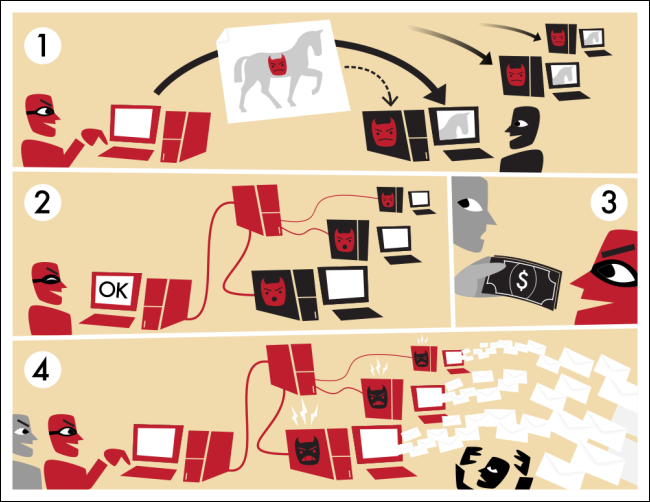
\includegraphics[scale=0.6]{./fig/botnetshowcase.png}
  \caption{A botnet showcase. (1) The attacker spreads bots via an infection vector — e.g. a trojan horse. (2) The infected hosts join the botnet, being remotely controllable by the attacker, via a command\&control server. (3) The computational power of the botnet is rent, for wichever malicious purpose, making the attacker gaining a lot of profits. (4) The attacker instructs the botnet to perform a spamming campaign, as requested by its client.}
    \label{fig:botnet-showcase}
\end{figure}

The \textit{command and control (C\&C)} is the component responsible for the distribution of commands to bots. Botnets can be controlled in several different ways, depending on how C\&C is implemented. In its simplest form, the C\&C implements a \textit{centralized client-server architecture} (i.e. \textit{C\&C server}), where bots poll a web server for commands to execute. Such a botnet is easy to stop — monitor what web servers a bot is connecting to, then take them down and causing the bots to be unable to communicate with the attacker. In a more advanced form, it implements a \textit{peer-to-peer (P2P) architecture} (i.e. \textit{C\&C node}), where bots instruct (are instructed by) other nearby bots, thus providing the botnet with a high degree of availability and redundancy. Since no single point of control can be identified, such botnets cannot be neutered only by disabling specific nodes. Therefore, defensive strategies are based on issuing fake commands or by isolating the bots from each other. Things are made harder since botnets started communicating, not only through encrypted channels, but via anonimous networks — such as Tor — where it’s theoretically impossible to figure out the botnet topology.

The \textit{ZeroAccess botnet} is an important example. The ZeroAccess botnet is one of the largest known botnets with a population upwards of 1.9 million computers, generating profits through Bitcoin mining and click frauds \cite{zeroaccess-symantec-blog,zeroaccess-symantec-definition}.
A key feature of the ZeroAccess botnet is its use of a P2P based C\&C, making it highly resistant to any take-down attempts.

\section{Architecture}
\label{sec:architecture}

The botnet implements the architecture showned in \Cref{fig:botnet-architecture}, where the C\&C layer is both implemented by a centralized web server exposing REST interfaces, and simulated by the local file system providing JSON files mimicking web server's responses.

\begin{figure}[tp]
  \centering
  \includegraphics[scale=0.25]{./fig/architecture.eps}
  \caption{The botnet architecture. In the \textit{real scenario}, the bot interacts with a C\&C layer implemented by web server exposing REST APIs — namely a controller. In the \textit{test scenario}, the bot interacts with the local file system, simulating controller's responses with local JSON files. In both scenarios, the bot is configured by a local configuration file, may produce local logs and performs attacks via the Internet.}
    \label{fig:botnet-architecture}
\end{figure}

In a \textit{real scenario}, the bot interacts with the web server through its REST APIs, whilst in a \textit{test scenario} it interacts with the local file system providing JSON files that simulates controller's responses.
In both scenarios, the controller is defined giving three interfaces: the \textit{init interface} is the one from which the bot loads the configuration to join the botnet; the \textit{command interface} from which the bot loads commands to execute; the \textit{log interface} is the one that the bot submits reports to.

Such a model makes our bot is suitable both for \textit{local testing}, where interfaces are local files, and \textit{real bot-controller interaction}, where interfaces are web interfaces.
In the following we often says "the bot receives from the controller" and "the bot sends to the controller", meaning without distinction whetere the bot is interacting with the controller in the real or testing scenario.

The bot is configured providing a YAML configuration file and executes commands given in JSON format. Both can be produced by convenient web-based interfaces presented in \ref{sec:configuration-wui} \ref{sec:commands-wui}, respectively.

\section{Bot}
\label{sec:bot}

The bot life cycle is modeled as a Finite State Automaton (FSA) with the state space defined as follows and depicted in \ref{fig:bot-fsa}.

\begin{figure}[tp]
  \centering
  \includegraphics[scale=0.09]{./fig/FSA.eps}
  \caption{The bot's finite state automaton (FSA).}
    \label{fig:bot-fsa}
\end{figure}

\begin{description}
  \setlength\itemsep{1em}

  \item[INIT] the bot generates a unique identifier in the form \texttt{MAC:JVM}, where \texttt{MAC} is the local MAC address and \texttt{JVM} is the name of the Java Virtual Machine currently running the bot; it then allocates basic resources (e.g. shutdown hooks for resource releasing); it tries to join a botnet using the specified list of controllers.
  Errors in this state are considered fatal, so they would cause bot termination. The pseudocode of this state is shown in \cref{alg:state-init-pseudocode}.

  \item[EXECUTION] the bot polls the controller for the next command; it waits a delay before command execution (if required); it executes the command; it produces the report and sends it to the controller (if required); it waits for the next polling.
  Errors in this state are considered warnings: they are handled and never cause bot termination. The pseudocode of this state is shown in \Cref{alg:state-execution-pseudocode}.

  \item[SLEEP] no reports are sent to the controller nor attacks are executed. The bot polls the controller for the next command, waiting for a \texttt{WAKEUP} (it would transit to state \texttt{EXECUTION}) or a \texttt{KILL} (it would transit to state \texttt{DEAD}).
  In this state errors are considered warning: they are handled and never cause bot termination. The pseudocode of this state is shown in \Cref{alg:state-sleep-pseudocode}.

  \item[DEAD] attacks are unscheduled, resources are released and the bot terminates. In this state all errors are ignored, because no one of them could never compromise the state purpose. The pseudocode of this state is shown in \Cref{alg:state-dead-pseudocode}.

\end{description}

\bigskip

\begin{algorithm}[H]
  \SetAlgoNoLine
  $mac \leftarrow$ getMACAddress() \\
  $jvm \leftarrow$ getJVMName() \\
  $id \leftarrow$ concat($mac$,$jvm$) \\
  setBotId($id$)
  $controller \leftarrow$ None \\
  $joined \leftarrow$ False \\
  $controllerIdx \leftarrow$ 0 \\
  $reconnections \leftarrow$ 0 \\
  $maxReconnections \leftarrow$ getBotConfig(RECONNECTIONS) \\
  $reconnectionWaitInterval \leftarrow$ getBotConfig(RECONNECTION-WAIT) \\
  \While{ not $joined$ } {
    $currentController \leftarrow$ getBotConfig(CONTROLLERS,$controllerIdx$)
    \If{ canLoadConfig($currentController$) } {
      loadConfig($currentController$)
      $controller \leftarrow$ $currentController$
      $joined \leftarrow$ True
    } \Else {
      $reconnections \leftarrow reconnections + 1$
      \If { $reconnections <= maxReconnections$ } {
        $reconnectionWait \leftarrow$ randomWithin($reconnectionWaitInterval$) \\
        wait($reconnectionWait$)
      } \Else {
        $controllerIdx \leftarrow controllerIdx + 1$
      }
    }
  }
  \caption{Pseudocode for state \texttt{INIT}}
  \label{alg:state-init-pseudocode}
\end{algorithm}

\bigskip

\begin{algorithm}[H]
  \SetAlgoNoLine
  $controller \leftarrow$ getBotConfig(CONTROLLER) \\
  $pollWaitInterval \leftarrow$ getBotConfig(POLL-WAIT) \\
  $reportType \leftarrow$ getBotConfig(REPORT-TYPE) \\
  $command \leftarrow$ getNextCommand() \\
  \If{requiresDelay($command$)} {
    $cmdDelayInterval \leftarrow$ getCommandParam($command$,DELAY-INTERVAL) \\
    $cmdDelay \leftarrow$ randomWithin($cmdDelayInterval$) \\
    wait($cmdDelay$)
  }
  executeCommand($command$)
  \If{requiresReport($command$)} {
    generateReport($reportType$) \\
    sendReportTo($controller$)
  }
  $pollWait \leftarrow$ randomWithin($pollWaitInterval$) \\
  wait($pollWait$)
  \caption{Pseudocode for state \texttt{EXECUTION}}
  \label[alg]{alg:state-execution-pseudocode}
\end{algorithm}

\bigskip

\begin{algorithm}[H]
  \SetAlgoNoLine
  $controller \leftarrow$ getBotConfig(CONTROLLER) \\
  $pollWaitInterval \leftarrow$ getBotConfig(POLL-WAIT) \\
  $reportType \leftarrow$ getBotConfig(REPORT-TYPE) \\
  $command \leftarrow$ getNextCommand() \\
  \If{$command =$ WAKEUP $command =$ KILL} {
    \If{requiresDelay($command$)} {
      $cmdDelayInterval \leftarrow$ getCommandParam($command$,DELAY-INTERVAL) \\
      $cmdDelay \leftarrow$ randomWithin($cmdDelayInterval$) \\
      wait($cmdDelay$)
    }
  }
  executeCommand($command$)
  $pollWait \leftarrow$ randomIn($pollWaitInterval$) \\
  wait($pollWait$)
  \caption{Pseudocode for state \texttt{SLEEP}}
  \label[alg]{alg:state-sleep-pseudocode}
\end{algorithm}

\bigskip

\begin{algorithm}[H]
  \SetAlgoNoLine
  $waitJobs \leftarrow$ getBotConfig(WAIT-JOBS) \\
  stopScheduler($waitJobs$) \\
  freeScheduler() \\
  freeIOResources() \\
  interruptBotLoop() \\
  executeShutdownHooks() \\
  exit()
  \caption{Pseudocode for state \texttt{DEAD}}
  \label[alg]{alg:state-dead-pseudocode}
\end{algorithm}

\section{Controller}
\label{sec:controller}

The controller is a centralized web server exposing the HTTP REST interfaces  described in \Cref{tab:controller-rest} to interact with the public audience, the attacker and the bot.
In particular, the public audience is provided with the \textit{fake landig page} in \Cref{fig:controller-fake-landingpage}, the attacker with the  \textit{botnet management dashboard} in \Cref{fig:controller-botnet-dashboard} and the bot with a subset of \textit{HTTP REST APIs}.

\begin{table}%
\caption{Controller HTTP REST API}
\label{tab:controller-rest}
\begin{minipage}{\columnwidth}
\begin{center}
\begin{tabular}{clcl}
  \toprule
  METHOD & RESOURCE & CONTENT & DESCRIPTION \\
  GET    & /        & HTML    & Shows the fake landing page. \\
  GET    & /admin   & HTML    & Shows the botnet management dashboard. \\
  GET    & /init    & JSON    & Returns the controller configuration.   \\
  GET    & /command & JSON    & Returns the next command to execute. \\
  POST   & /report  & JSON    & Saves the bot report. \\
  \bottomrule
\end{tabular}
\end{center}
\end{minipage}
\end{table}

The content of the landing page must be such as to arouse in visitors both trust and indifference. In this way the visitor does not alarm and pass through without having any interest to further explore the website.

\begin{figure}[tp]
  \centering
  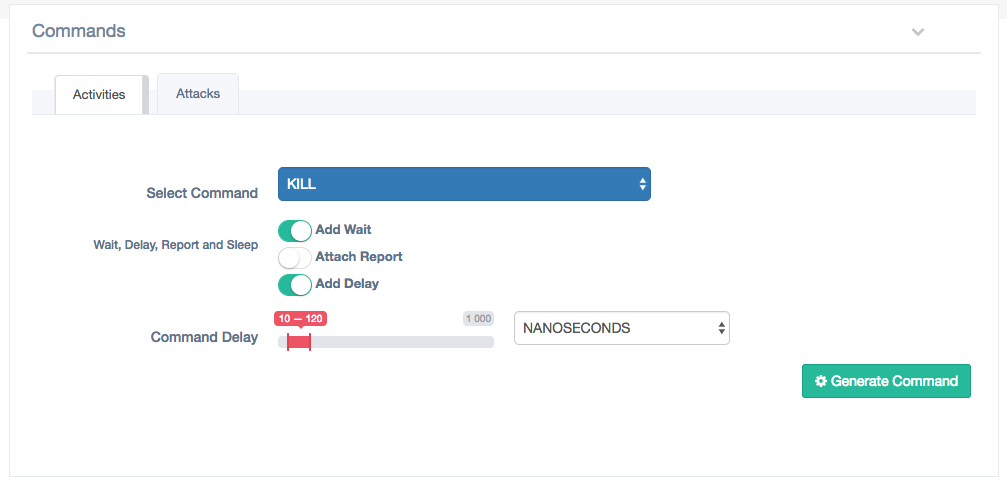
\includegraphics[scale=0.2]{./fig/commandsWUI.png}
  \caption{The fake landing page at \texttt{/index.html}.}
    \label{fig:controller-fake-landingpage}
\end{figure}

The botnet management dashboard provides the attacker with convenient forms to generate bot configurations, to generate and submit both controller configurations and commands. Furthermore, all saved bot reports are stored in \texttt{/controller/data/report} as \texttt{report.\$\{botIP\}.json}.

\begin{figure}[tp]
  \centering
  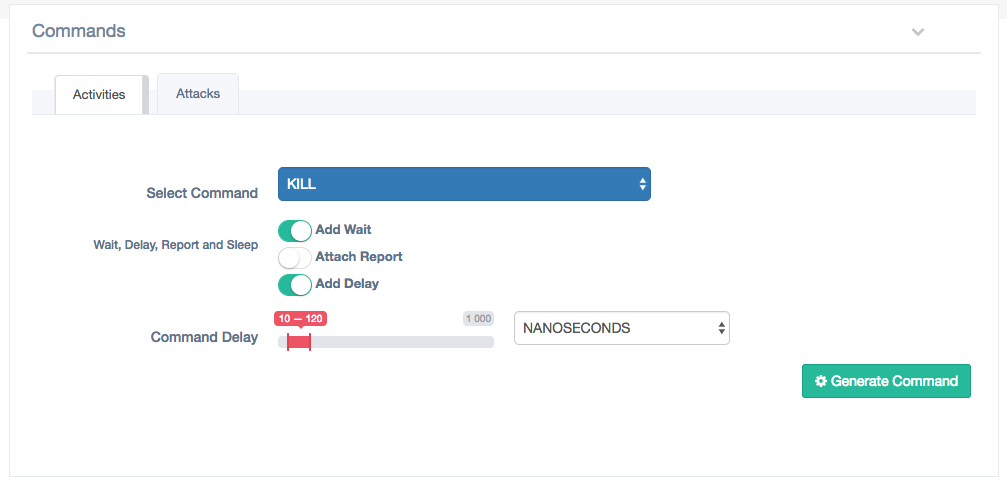
\includegraphics[scale=0.2]{./fig/commandsWUI.png}
  \caption{The botnet dashboard at \texttt{/admin.html}.}
    \label{fig:controller-botnet-dashboard}
\end{figure}

\section{Configuration}
\label{sec:configuration}

The bot behaviour is ruled both by a \textit{local configuration} and by a \textit{controller-specific configuration}. The former is a fully customizable local YAML file; the latter is given as a JSON response to \texttt{GET /init} loaded when joining the botnet.
When no local configuration is specified, the bot looks for a YAML file named \texttt{config.yaml} in the present working directory. If not there, the bot loads the default configuration , which is hardly wired in code. For details about how to submit a custom configuration, please refer to \ref{sec:usage}.

We now show the configuration components, the YAML configuration schema to express them and a tool to generate configurations.

\begin{description}
  \setlength\itemsep{1em}

  \item[cnfInfo] if true, reports include the current bot configuration.

  \item[tgtInfo] if true, reports include details about the targets to attack.

  \item[sysInfo] if true, reports include details about the localhost system.

  \item[netInfo] if true, the bot report includes details about the network the localhost is attached to.

  \item[polling] period between consecutive requests to the controller for the next command to execute. The polling period is a random amount of time within a certain time interval. The randomness of period guarantees a greater variance in bots behaviour. Typically the period depends on the botnet needs. However, it is good practice not to set a too short period to ensure the concealment of the bot on the infected system\footnote{the default configuration provides a 10-15 seconds polling period for testing convenience.}.

  \item[reconnections] number of times the bot tries to connect to an unreacheable controller.

  \item[reconnectionWait] period between reconnections. The reconnection period is a random amount of time within a certain time interval. The period randomness guarantees a greater variance in bots behaviour. Such a period depends on the known controller availability.

  \item[proxy] HTTP proxy behind which the bot contacts remote controllers and targets. The default configuration has no proxy.

  \item[sleep] calendar for the sleeping mode. The default configuration has no sleep calendar.

  \item[authentication] a list of key-value pairs used as HTTP headers during bot-controller interactions. A minimal authentication setting should provide at least the \texttt{User-Agent}, but many more can be added, according to botnet security needs.

  \item[controllers] list of controllers to contact. The default configuration has an empty list of controllers. Each controller inherits (and may overwrite) the properties \texttt{polling, reconnections, reconnectionWait, proxy, sleep, authentication}.

\end{description}

The configuration is given in YAML format, with default values as comments. The schema shows some non primitive data types that deserves further attention.

\begin{verbatim}
  cnfInfo: True|False # True
  tgtInfo: True|False # True
  sysInfo: True|False # True
  netInfo: True|False # True
  polling: time-expression # 10-15:SECONDS
  reconnections: integer in [0,65535] # 0
  reconnectionWait: time-expression # 10-15:SECONDS
  proxy: proxy-expression # none
  sleep: cron-expression  # Null
  authentication: dict-object # {}
  controllers: [controller-object] # []
\end{verbatim}

A \texttt{time-expression} represents a temporal interval — e.g. a value in seconds between 3 and 5 seconds. This expression is a string in the form \texttt{min-max:unit}, where \texttt{min} is a positive long, \texttt{max} is a positive long greater than or equal to \texttt{min}, and \texttt{unit} is the string representation of a standard Java TimeUnit\footnote{i.e. NANOSECONDS, MICROSECONDS, MILLISECONDS, SECONDS, MINUTES, HOURS, DAYS.}. If \texttt{min} and \texttt{max} are both equal to a positive long \texttt{amount}, the time interval could be representaed both by the redundant expression \texttt{amount-amount:unit} and by the more compact expression \texttt{amount:unit}.

A \texttt{proxy-expression} represents a HTTP proxy — e.g. the proxy 123.123.123.123 with port 3000. This expression is a string in the form \texttt{address:port}, where \texttt{addres} is an IPv4 address and \texttt{port} is a port number. The expression can also be a string \texttt{none}, meaning that no proxy should be used, and \texttt{null}, meaning that any default proxy should be used.

A \texttt{cron-expression} represents a calendar — e.g. every Wednesday between 10 PM and 11PM. This expression is a standard Unix CRON expression. For details about the standard, please refer to \cite{cron-expression}.

A \texttt{dict-expression} represents a dictionary between strings and strings — e.g. "prop1" set to "val1".

A \texttt{controller-object} represents a bot controller — e.g. a controller with init interface X command interface Y and log interface Z. A controller is expressed in the following form:

\begin{verbatim}
  init: resource-expression
  cmd:  resource-expression
  log:  resource-expression
  polling: time-expression # 10-15:SECONDS
  reconnections: integer in [0,65535] # 0
  reconnectionWait: time-expression # 10-15:SECONDS
  proxy: proxy-expression # none
  sleep: cron-expression  # Null
  authentication: dict-object # {}
\end{verbatim}

where a \texttt{resource-expression} represents a readable local or remote resource — i.e. a standard file pathname or a remote Web URL.

\subsection{Sample configuration}
\label{sec:sample-configuration}

Here we show a sample configuration for reader's convenience. Other sample configurations can be found in \texttt{data/samples/configurations}.

\begin{verbatim}
  cnfInfo: True
  tgtInfo: False
  sysInfo: True
  netInfo: False
  polling: 10-15:SECONDS
  reconnections: 3
  reconnectionWait: 3-5:SECONDS
  proxy: 123.123.123.123:3000
  sleep: * * * SAT-SUN * ?
  authentication:
    User-Agent: MyAwesomeBot
    Authentication: Basic 123456789
    BotID: 270690
  controllers:
    - init: data/samples/controllers/1/botinit.json
      command: data/samples/controllers/1/botcmd.json
      log: data/samples/controllers/1/botlog.json
    - init: data/samples/controllers/2/botinit.json
      command: data/samples/controllers/2/botcmd.json
      log: data/samples/controllers/2/botlog.json
\end{verbatim}

\subsection{Configuration WUI}\label{sec:configuration-wui}


\begin{figure}[tp]
  \centering
  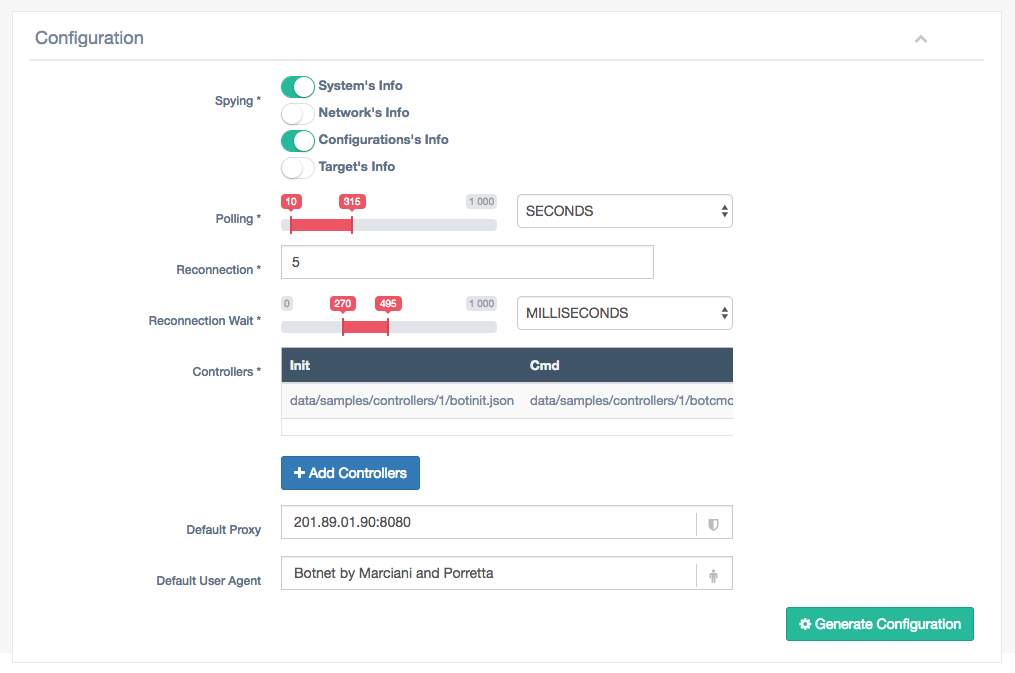
\includegraphics[scale=0.45]{./fig/configurationWUI.png}
  \caption{The Web User Interface to build configurations.}
    \label{fig:configuration-wui}
\end{figure}

\textcolor{green}{\lipsum[1]}

\section{Commands}
\label{sec:commands}

In the following we list all commands with the corresponding JSON schema.
For sake of synthesis, we indicate in a pretty custom way (pseudo-JSON) both the optional fields and the non primitive data types.

For example, in the following pseudo-JSON: \texttt{f1} is a mandatory field with value \texttt{v1}; \texttt{f2} is a mandatory field with domain in ad-hoc data type \texttt{T}; \texttt{f3} is an optional field with domain \texttt{T} and default value \texttt{default}; \texttt{f4} and \texttt{f5} are optional fields going together with domain \texttt{T} and default value \texttt{default}.

\begin{verbatim}
  {
    "f1": "v1",
    "f2": T,
    ("f3": T (default)),
    (
      "f4": T (default),
      "f5": T (default)
    )
  }
\end{verbatim}

In the command listed below there are non primitive data types. Some of them have been already mentioned in \ref{sec:configuration}. We report here them too, for reader's convenience.

\begin{description}
  \setlength\itemsep{1em}

  \item[time-expression] represents a temporal interval — e.g. a value in seconds between 3 and 5 seconds. This expression is a string in the form \texttt{min-max:unit}, where \texttt{min} is a positive long, \texttt{max} is a positive long greater than or equal to \texttt{min}, and \texttt{unit} is the string representation of a standard Java TimeUnit\footnote{i.e. NANOSECONDS, MICROSECONDS, MILLISECONDS, SECONDS, MINUTES, HOURS, DAYS.}. If \texttt{min} and \texttt{max} are both equal to a positive long \texttt{amount}, the time interval could be representaed both by the redundant expression \texttt{amount-amount:unit} and by the more compact expression \texttt{amount:unit}.
  For example, the following are valid expressions:

  \begin{verbatim}
    3-5:SECONDS
  \end{verbatim}

  and

  \begin{verbatim}
    10:SECONDS
  \end{verbatim}

  \item[proxy-expression] represents a HTTP proxy — e.g. the proxy 123.123.123.123 with port 3000. This expression is a string in the form \texttt{address:port}, where \texttt{addres} is an IPv4 address and \texttt{port} is a port number. The expression can also be a string \texttt{none}, meaning that no proxy should be used, and \texttt{null}, meaning that any default proxy should be used.
  For example, the following are valid expressions:

  \begin{verbatim}
    123.123.123:3000
  \end{verbatim}

  and

  \begin{verbatim}
    none
  \end{verbatim}

  \item[web-expression] represents a Web URL — http://www.google.com. Pay attention that it is necessary to specify the HTTP protocol.
  For example, the following is valid expressions:

  \begin{verbatim}
    http://www.google.com
  \end{verbatim}

  whereas the following is not

  \begin{verbatim}
    www.google.com
  \end{verbatim}

  \item[dict-expression] represents a dictionary between strings and strings — e.g. "prop1" set to "val1".
  For example, the following is valid expressions:

  \begin{verbatim}
    {
      "prop1": "val1",
      "prop2": "val2"
    }
  \end{verbatim}

  \item[attack-object] represents a target of a HTTP attack — e.g. a GET attack to http://www.google.com.
  If specified, \texttt{proxy} is the HTTP proxy to attack through. If set to \texttt{null}, it is the default proxy (see \ref{sec:configuration}).
  If specified, \texttt{properties} are the HTTP request parameters to attack with.
  If specified, \texttt{executions} indicates how many attack executions need to be scheduled interleaved by the secified \texttt{period}.

  \begin{verbatim}
  {
    "method": value in [GET,POST],
    "target": web-expression,
    ("proxy": proxy-expression (null)),
    ("properties": dict-expression ({})),
    (
      "executions": integer in [1,65535] (1),
      "period": time-expression (null)
    )
  }
  \end{verbatim}

  For example, the following are valid expressions:

  \begin{verbatim}
  {
    "method": "GET",
    "target": "http://www.google.com"
  }
  \end{verbatim}

  and

  \begin{verbatim}
  {
    "method": "GET",
    "target": "http://www.google.com",
    "proxy": "123.123.123:3000",
    "properties": map-expression {
      "User-Agent": "CustomUserAgent"
    },
    "executions": 3,
    "period": "3-5:SECONDS"
  }
  \end{verbatim}

\end{description}

Every command starts with a field pointing out the command scope, and terminates with the expected parameters.
Every command\footnote{with the exception of command \texttt{NONE} having no fields, and command \texttt{REPORT} having no optional field \texttt{report}.}  has a optional fields \texttt{delay} and \texttt{report}.

If \texttt{delay} is specified, the command will be executed after a random amount of time within the given interval; if not, the command will be executed immediately. This optional field has been added to command schema because in some real scenarios could be useful to specify a variance component.

If \texttt{report} is specified and set to \texttt{true}, the bot will send the report back to the controller, once the command has been executed. If set to \texttt{false}, no report will be sent back to the controller. This optional field has been added to the command schema as a shortcut for whichever command followed by the \texttt{REPORT} command. Sometimes, as stated in \cite{build-your-own-botnet}, the reporting procedure is embedded in every bot-controller interaction, as a bot response to command requests. We avoided such an approach because (i) it does not scale with botnet dimension\footnote{it would sound somehow as a DDoS suicide.} and (ii) the local host analysis is an action in itself, not strictly related to the curretn executing command\footnote{for example, keylogging is not a bot response to controller's requests, but an additional, though frequent, function.}.

\begin{description}
  \setlength\itemsep{1em}

  \item[ATTACK-HTTP] schedules all the specified HTTP \texttt{attacks}.

  \begin{verbatim}
  {
    "command": "ATTACK_HTTP",
    "attacks": [ attack-object ],
    ("delay": time-expr (null))
  }
  \end{verbatim}

  \item[CALMDOWN] all attacks are unscheduled.
  If \texttt{wait} is true, it waits for for termination of currently executing attacks; if false, it kills them immediately.

  \begin{verbatim}
  {
    "command": "CALMDOWN",
    ("wait": boolean (false)),
    ("delay": time-expr (null))
  }
  \end{verbatim}

  \item[KILL] the bot is killed, that is alla attacks are unscheduled and it transit to state \texttt{DEAD} for resource releasing.
  If \texttt{wait} is true, it waits for for termination of currently executing attacks; if false, it kills them immediately.

  \begin{verbatim}
  {
    "command": "KILL",
    ("wait": boolean (false)),
    ("delay": time-expr (null))
  }
  \end{verbatim}

  \item[NONE] instructs the bot to do nothing, that is to neither change its executions flow nor send any report. In particular, both the null (empty file) and the empty command (empty JSON, i.e. {}) are equivalent to \texttt{NONE}.

  \begin{verbatim}
  {
    "command": "NONE"
  }
  \end{verbatim}

  \item[REPORT] the bot sends the report to the controller.

  \begin{verbatim}
  {
    "command": "REPORT",
    ("delay": time-expr (null))
  }
  \end{verbatim}

  \item[RESTART] all attacks are unscheduled, the bot transits to state \texttt{INIT} trying to contact the controller with \texttt{resource} as its init-interface.
  If \texttt{wait} is true, it waits for for termination of currently executing attacks; if false, it kills them immediately.

  \begin{verbatim}
  {
    "command": "RESTART",
    "resource": resource-expr,
    ("wait": boolean (false)),
    ("delay": time-expr (null))
  }
  \end{verbatim}

  \item[SAVE-CONFIG] the currently loaded bot configuration is locally saved as default configuration.

  \begin{verbatim}
  {
    "command": "SAVE_CONFIG",
    ("delay": time-expr (null))
  }
  \end{verbatim}

  \item[SLEEP] all attacks are suspended and the bot transits to state \texttt{SLEEP}. If a \texttt{timeout} si specified the command \texttt{WAKEUP} is internally invoked after a random amount of time within the specified interval.

  \begin{verbatim}
  {
    "command": "SLEEP",
    ("timeout": time-expr (null)),
    ("delay": time-expr (null))
  }
  \end{verbatim}

  \item[UPDATE] the bot configuration is updated with the properties specified in \texttt{settings}. This command is tipically used to update the property \texttt{sleep} that sets the sleep mode.

  \begin{verbatim}
  {
    "command": "UPDATE",
    "settings": map-expr,
    ("delay": time-expr (null))
  }
  \end{verbatim}

  \item[WAKEUP] if the bot is in state \texttt{SLEEP}, it lets scheduled attacks be able to fire again and transits to state \texttt{EXECUTION}.

  \begin{verbatim}
  {
    "command": "WAKEUP",
    ("delay": time-expr (null))
  }
  \end{verbatim}

\end{description}

\subsection{Commands WUI}
\label{sec:commands-wui}

\textcolor{green}{\lipsum[1]}

\begin{figure}[tp]
  \centering
  
\includegraphics{./fig/acmlarge-mouse}
  \caption{\textcolor{green}{The Web User Interface to build commands.}}
    \label{fig:commands-wui}
\end{figure}

\textcolor{green}{\lipsum[1]}

\section{Reports}
\label{sec:reports}

The bot can send to the controller reports containing \textit{current bot configuration}, \textit{scheduled attacks}, \textit{local system analysis} and \textit{local networks analysis}. Each section is attached to reports, if requested in configuration (see options \texttt{cnfInfo}, \texttt{tgtInfo}, \texttt{sysInfo} and \texttt{netInfo} in Section~\ref{sec:configuration}). Since the first two sections are self-explanatory, we focus here only on local system and networks analysis.\\

The \textit{local system analysis} includes the following components:
\begin{description}
  \setlength\itemsep{1em}
    \item [browsers] list of browsers installed on system. Browsers are detected by parsing the report of installed applications, returned by system's command of specific OS (e.g. Linux command: "\textit{dpkg -l}").
	\item [hostName] name associated with the host machine.
	\item [kernelVersion] version of the system kernel.
	\item [osArch] name of the system's architecture.
  	\item [osName] name of the operating system.
  	\item [osVersion] version of the operating system.
  	\item [userName] name of the active user on the host.
\end{description}
\;

An example of system analysis is the following:
\begin{description}
	\item 
		\begin{verbatim}
		{
		  "Browsers" : "Google Chrome; Safari;",
		  "HostName" : " MacBook Pro di Michele",
	 	"KernelVersion" : " Darwin 15.5.0",
	 	"OsArch" : "x86_64",
		  "OsName" : "Mac OS X",
		  "OsVersion" : "10.11.5",
		  "UserName" : " Michele Porretta (micheleporretta)"
		}
		\end{verbatim}
\end{description}

The \textit{local networks analysis} includes the following components:

\begin{description}
  \setlength\itemsep{1em}
  \item [Mac] Mac Address.
  \item [Ip] Ip Address.
  \item [CurrentNetworkInfo] List of network interfaces with their details. This report is produced by following system's command to the \textit{Unix-Like} machines:
	\begin{verbatim}
		ifconfig
	\end{verbatim}
	And with the following command for \textit{Windows NT} machines: 
	\begin{verbatim}
		ipconfig
	\end{verbatim}
  \item [NetworkStatistics] Statistics about network traffic, classified by protocol. This report is produced by the following command: 
	\begin{verbatim}
		netstat -s			
	\end{verbatim}
	Where \textit{Netstat} is a command-line utility useful  for checking network configuration and activity.
  \item [TcpConnections] Active Tcp connections. This report is produced by the following command: 
  	\begin{verbatim}
		netstat -p tcp  		
  	\end{verbatim}
  \item [UdpConnections] Active Udp connections. This report is produced by the following command: 
  	\begin{verbatim}
		netstat -p udp  		
  	\end{verbatim}

 \end{description}

Notice that the use of \texttt{netInfo} may slow down the execution, as it scans all the active \textit{TCP} and \textit{UDP} connections.

An example of network analysis is the following:

\begin{description}
	\item 
		\begin{verbatim}
		{
		  "MAC" : "6C-D2-C4-76-FB-24",
		  "ip" : "10.224.219.219",
	 	"currentNetworkInfo" : "[ network info ]",
	 	"networkStatistics" : "[ statistics ]",
	 	"tcpConnections" : "[ active tcp connections ]",
	 	"udpConnections" : "[ active udp connections ]"
		}
	\end{verbatim}
\end{description}
\section{Implementation}
\label{sec:implementation}

The bot has been realized as a Java\footnote{Oracle Java SE 8} desktop application, packaged with Maven into a self-contained\footnote{fat jar encapsulating all external dependencies.} jar with shrunk and obfuscated code.

Basically, the bot implements the finite state automaton (\ref{sec:bot}) and the functionalities required for configuration parsing (\ref{sec:configuration}), commands execution (\ref{sec:commands}) and logging. All functionalities has been tested carefully against 123 total JUnit tests.

\textcolor{green}{WEB INTERFACE IMPLEMENTATION \lipsum[1]}

Our bot and web user interfaces leverage some of well known technologies. Here we present them, giving an idea about how they have been used in our implementation. The reader may refer to the open source code of the project and the corresponding Javadocs to get into implementation details.

\begin{description}
  \setlength\itemsep{1em}

  \item[QUARTZ] job scheduling framework developed by the Terracotta Inc \cite{quartz-scheduler}.
  It is a widely adopted solution to support process workflow and system management in enterprise applications.
  In our application it is used to implement the bot thread pool for both attacks and sleep mode scheduling.

  \item[LOG4J2] logging framework developed by the Apache Software Foundation \cite{log4j2}.
  It is a de facto standard for logging in Java\footnote{together with its main competitor, Logback.}, tipically used as a SLF4J binding\footnote{SLF4J is a widely adopted Java logging facade.}.
  In our application, it is used both for console and file logging.

  \item[COMMONS CLI] command line parsing framework developed by the Apache Software Foundation as a part of the bigger Jakarta project\cite{commons-cli}.
  It is a well known solution for argument parsing in CLI based Java applications.

  \item[JACKSON] serialization framework developed by the Fasterxml team \cite{jackson}.
  It supports most of the widespread serialization format, such as JSON, XML, YAML and so on.
  In our application it is used to serialize/deserialize configuration (in YAML) and commands (in JSON).

  \item[LOMBOK] framework of annotations for the encapsulation of boilerplates and simple patterns \cite{lombok}.
  In our application it is used to generate constructors getters/setters toString/hashCode methods. As such a generation is evaluated at compile time, the code of entity classes is considerably reduced.

  \item[BOOTSTRAP] \textcolor{green}{\lipsum[1]}

  \item[JQUERY] \textcolor{green}{\lipsum[1]}

\end{description}


\subsection{Concealment}
\label{sec:concealment}

Since the bot is a malware, its first priority is not to be discovered by the victim's system. Just like any malware, bots should be easily distributed, act covertly and evade the health checks of the infected system. The concealment can be achieved, in the first instance, by making the code minimal, efficient and obfuscated.

\textit{Code minimization} allows to distribute the bot in a small sized package, which is easy to conceal in an infection vector, easy to trasmit and whose installation on the system goes unnoticed.
\textit{Code efficiency} allows the bot to act in a minimally invasive way in terms of memory usage, access to local resources, external communications and sub-processes creation.
\textit{Code obfuscation} allows the bot to evade traditional health checks based on code patterns analysis. As a beneficial side effect, an obfuscation dictionary with short words can assist code minimization.

All of these aspects have been implemented leveraging \textit{ProGuard}, the most popular Java bytecode optimizer developed by the GuardSquare Inc. \cite{proguard}. This tool realizes code shrinking, optimization and obfuscation. It can make Java applications up to 90\% smaller, up to 20\% faster and protected against reverse engineering\cite{guardsquare}.

In our application, ProGuard has been embedded into the Maven packaging life-cycle via an ad-hoc plugin \cite{proguard-maven-plugin}. The adopted configuration of ProGuard behaviour can be found in \texttt{config.pro}. From this configuration a conservative approach may be noticed. The widespread use of reflection, serialization and annotations in the framework the bot code depends on, makes it necessary to limit both the shrinking and the obfuscation of these frameworks. A deeper code inspection on these frameworks would allow a more aggressive approach, thus obtaining a more minimized and obfuscated code. \footnote{Code obfuscation is subjected to a crucial tradeoff, because the excessive or naive code obfuscation may have collateral side effects. The obfuscation of the whole legitimate code may arouse suspicion of a meticolous checks, because only a legitimate program of high industrial value has no dependency on legitimate clear code. On the other hand, legitimate code letting guess actions of malicious program should never left clear.}.


\subsection{Logging}
\label{sec:logging}

Our bot records events both on console and file adopting a logging discipline that depends on the chosen execution mode. The \texttt{default} mode prints in console the strictly relevant output and produces log files. The \texttt{trace} mode prints in console a detailed tracing output and produces log files. The \texttt{silent} mode does neither print anything in console nor produce any log file.
To run the program in one of these modes, specify the corresponding option, as indicated in \ref{sec:usage}.

Console logging prints events on the standard output\footnote{standard error is never used, neither in case of warnings nor errors.}.
File logging deals with three types of events: it appends commands-related events on \texttt{data/log/commands.log}, attacks-related ones on \texttt{data/log/attacks.log} and report-related ones on \texttt{data/log/reports.log}. These two files are emptied every time the bot is started.

A general log message printed to console has the following pattern

\begin{verbatim}
  [timestamp] [tread-name] [log-level] [class] [method] - [message]
\end{verbatim}

A log message on file about commands has the following pattern

\begin{verbatim}
  [timestamp] Received [COMMAND] with [PARAMS] from C&C at [CC-RESOURCE]
\end{verbatim}

A log message on file about attacks has the following pattern

\begin{verbatim}
  [timestamp] Launching HTTP attack: [HTTP-METHOD] [TARGET] ([ITER]/[ITERS])
              behind proxy [ADDR:PORT] with request params [HTTP-REQUEST-PROPS]
\end{verbatim}

A log message on file about reports has the following pattern

\begin{verbatim}
  [timestamp] Report sent to C&C at [CC-RESOURCE] [REPORT]
\end{verbatim}

\section{Usage}
\label{sec:usage}

The bot can be run as a Java project inside an IDE, as a Maven project or as a self-contained Jar.
In a real scenario, the program would be delivered via an infected file as a self-contained, minimized and obfuscated Jar. Therefore, here, we will show only this compilation and execution method.
The controller can be built and run as a usual Node.js application packaged with NPM.
The reader may refer to the \texttt{README} file for details on other compilation and execution methods.

In the following, we assume that the execution environment is provided with JDK SE 8.* \cite{jdk}, Maven 3.*, \cite{maven}), Node.js \cite{nodejs} and NPM \cite{npm}. We also assume that an Internet connection is available and that both the Jar execution and whichever referenced file do not require any root rights.

\subsection{Bot compilation and execution}
\label{sec:bot-compilation-execution}

The bot is compiled into a self-contained Jar using the Maven packaging procedure, running the command:

\begin{verbatim}
  $[bot-dir]> mvn package -P optimize,skip-tests
\end{verbatim}

The previous command executes the packaging using both the profile \texttt{optimize} and \texttt{skip-tests}.

Since the bot code should always be optimized — i.e. minimized and obfuscated — we recommend providing this stage, activating the \texttt{optimize} profile. The code optimization is realized by running Proguard in the background (downloadable from \cite{proguard}) and may slow down the compilation. If the execution environment doesn't require code optimization, or some compilation speed up is desidered, simply omit the corresponding profile.

Since the project involves more than one hundred JUnit tests, we recommend skipping them to speed up compilation, activating the \texttt{skip-tests} profile. If you considered necessary to perform tests, simply omit the corresponding profile.

The compilation produces a Jar file \texttt{bot-1.0-optimized.jar} in the \texttt{target} folder. Since it is self-contained, it can be run in any system directory. In the following, we refer to this Jar with the shorter name \texttt{bot.jar}.

The bot provides the user with three execution mode: \texttt{default}, \texttt{trace} and \texttt{silent}, which are distinguished by the adopted logging discipline. The \texttt{default} mode prints in console the strictly relevant output and produces log files. The \texttt{trace} mode prints in console a detailed tracing output and produces log files. The \texttt{silent} mode does neither print anything in console nor produce any log file.
To run the program in one of these modes, specify the corresponding options \texttt{--trace} or \texttt{--silent}.

The program behaviour can be customized providing a custom YAML configuration file. If no configuration is specified, the program runs with default configuration. To run the program with custom configuration, specify the corresponding configuration, with the option \texttt{--config}.

To run the program with default configuration and default execution mode, run the command:

\begin{verbatim}
  $> java -jar bot.jar
\end{verbatim}

To run the program in \texttt{trace} execution mode, run the command:

\begin{verbatim}
  $> java -jar bot.jar --trace
\end{verbatim}

To run the program in \texttt{silent} execution mode, run the command:

\begin{verbatim}
  $> java -jar bot.jar --silent
\end{verbatim}

To run the program with custom configuration, run the command:

\begin{verbatim}
  $> java -jar bot.jar --config <CONFIG-FILE>
\end{verbatim}

The reader may refer to the program CLI helper for the options usage. We show here the helper output for reader's convenience.

\begin{verbatim}
  BOT version 1.0
  Team: ACM Rome Tor Vergata (http://acm.uniroma2.it)

  A bot showcase.
  Coursework in Computer Security 2015/2016

  usage: BOTNET [-c <CONFIG-FILE>] [-h] [-s] [-t] [-v]
   -c,--config <CONFIG-FILE>   Custom configuration.
   -h,--help                 Show app helper.
   -s,--silent               Activate silent mode.
   -t,--trace                Activate trace mode.
   -v,--version              Show app version.
\end{verbatim}

\subsection{Controller compilation and Execution}
\label{sec:controller-compilation-execution}

The controller is built as a usual NPM package, running the command:

\begin{verbatim}
  $[controller-dir]> npm install
\end{verbatim}

To start the controller, attaching it to the default port 3000, run the command:

\begin{verbatim}
  $[controller-dir]> node controller.js
\end{verbatim}

To start the controller, attaching it to the port \texttt{PORT} and allowing verbosity, run the command:

\begin{verbatim}
  $[controller-dir]> node controller.js --port [PORT] --verbose
\end{verbatim}

\section{Sample execution}
\label{sec:sample-execution}

We show here a sample execution to give the reader an idea about how everything works. We suggest the reader to refer to \cite{video-tutorial} to better undesrtand how configuration and commands could be conveniently generated.

In thi example, the bot is run in default mode with the following configuration:

\begin{verbatim}
  cnfInfo: True
  tgtInfo: True
  sysInfo: True
  netInfo: True
  controllers:
    - init: invalid/botinit.json
      command: invalid/botcmd.json
      log: invalid/botlog.json
    - init: controller/botinit.json
      command: controller/botcmd.json
      log: controller/botlog.json
  polling: 90-120:SECONDS
  reconnections: 3
  reconnectionWait: 2-5:SECONDS
  proxy: none
  userAgent: MyAwesomeBot
\end{verbatim}

Notice that the first specified controller is an invalid one - it mimics an unrecheable or compromised contoller.
The controller gives the bot the following \texttt{ATTACK-HTTP} command:

\begin{verbatim}
  {
    "command": "ATTACK_HTTP",
    "attacks": [
      {
        "method": "GET",
        "target": "http://www.twitter.com"
      },
      {
        "method": "GET",
        "target": "http://www.google.com",
        "proxy": "31.220.56.101:80",
        "properties": {
          "User-Agent": "MyAwesomeBot"
        },
        "executions": 3,
        "period": "10-15:SECONDS"
      }
    ]
  }
\end{verbatim}

followed by commands \texttt{REPORT} and \texttt{KILL}.
The following is the console output\footnote{classes and methods name indicated in \ref{sec:logging} have been omitted for better page formatting.}:

\begin{verbatim}
  18:03:59.537 [main] INFO Bot initialized with ID=20-68-9D-C3-76-EB-5261@debian
  18:03:59.540 [main] INFO Joining botnet...
  18:03:59.541 [main] INFO Loading bot configuration
               from C&C at invalid/botinit.json...
  18:03:59.549 [main] WARN Cannot connect to C&C at invalid/botinit.json,
               waiting for reconnection...
  18:03:59.551 [main] INFO Waiting for polling 2 SECONDS...
  18:04:01.552 [main] INFO Loading bot configuration
               from C&C at invalid/botinit.json...
  18:04:01.553 [main] WARN Cannot connect to C&C at invalid/botinit.json,
               waiting for reconnection...
  18:04:01.554 [main] INFO Waiting for polling 3 SECONDS...
  18:04:04.555 [main] INFO Loading bot configuration
               from C&C at invalid/botinit.json...
  18:04:04.556 [main] WARN Cannot connect to C&C at invalid/botinit.json,
               waiting for reconnection...
  18:04:04.557 [main] INFO Waiting for polling 2 SECONDS...
  18:04:06.557 [main] INFO Loading bot configuration
               from C&C at invalid/botinit.json...
  18:04:06.559 [main] WARN Maximum number of reconnections reached
               for C&C at invalid/botinit.json
  18:04:06.559 [main] INFO Loading bot configuration
               from C&C at controller/botinit.json...
  18:04:06.668 [main] INFO Bot is up and running
  18:04:06.755 [main] INFO Received command ATTACK_HTTP
               with params {attacks=[
               HttpAttack(method=GET, target=http://www.twitter.com,
               proxy=null, properties={},
               executions=1, period=null),
               HttpAttack(method=GET, target=http://www.google.com,
               proxy=31.220.56.101:80, properties={User-Agent=MyAwesomeBot},
               executions=3, period=10-15:SECONDS)]}
               from C&C at controller/botcmd.json
  18:04:06.756 [main] INFO Executing command ATTACK_HTTP
               with params {attacks=[
               HttpAttack(method=GET, target=http://www.twitter.com,
               proxy=null, properties={},
               executions=1, period=null),
               HttpAttack(method=GET, target=http://www.google.com,
               proxy=31.220.56.101:80, properties={User-Agent=MyAwesomeBot},
               executions=3, period=10-15:SECONDS)]}
               from C&C at controller/botcmd.json
  18:04:06.756 [main] INFO Scheduling attack against http://www.twitter.com...
  18:04:06.764 [main] INFO Attack scheduled
  18:04:06.764 [main] INFO Scheduling attack against http://www.google.com...
  18:04:06.776 [main] INFO Attack scheduled
  18:04:06.776 [main] INFO Waiting for polling 118 SECONDS...
  18:04:06.784 [BotPool_Worker-1] INFO Launching HTTP attack:
               GET http://www.twitter.com (1/1)
               behind proxy none
               with request params {User-Agent=MyAwesomeBot}
  18:04:06.784 [BotPool_Worker-2] INFO Launching HTTP attack:
               GET http://www.google.com (1/3)
               behind proxy 31.220.56.101:80
               with request params {User-Agent=MyAwesomeBot}
  18:04:20.766 [BotPool_Worker-3] INFO Launching HTTP attack:
               GET http://www.google.com (2/3)
               behind proxy 31.220.56.101:80
               with request params {User-Agent=MyAwesomeBot}
  18:04:34.766 [BotPool_Worker-4] INFO Launching HTTP attack:
               GET http://www.google.com (3/3)
               behind proxy 31.220.56.101:80
               with request params {User-Agent=MyAwesomeBot}
  18:06:04.780 [main] INFO Received command REPORT with params {}
               from CC at controller/botcmd.json
  18:06:04.780 [main] INFO Executing command REPORT with params {}
  18:06:04.843 [main] INFO Sending report to C&C at controller/botlog.json...
  18:06:04.846 [main] INFO Report sent to C&C at controller/botlog.json
  {
    "config" : {
      "cnfInfo" : true,
      "tgtInfo" : true,
      "sysInfo" : true,
      "netInfo" : true,
      "polling" : "90-120:SECONDS",
      "reconnections" : 3,
      "reconnectionWait" : "2-5:SECONDS",
      "proxy" : "none",
      "userAgent" : "MyAwesomeBot",
      "sleep" : null,
      "controllers" : [ {
        "init" : "controller/botinit.json",
        "command" : "controller/botcmd.json",
        "log" : "controller/botlog.json"
      } ]
    },
    "attacks-http" : [ ],
    "network-analysis" : "{MAC=20-68-9D-C3-76-EB, ip=127.0.1.1}",
    "system-analysis" : "{os=A cool OS, kernel=A cool kernel}"
  }
  18:06:04.847 [main] INFO Waiting for polling 91 SECONDS...
  18:07:35.851 [main] INFO Received command KILL with params {}
               from C&C at controller/botcmd.json
  18:07:35.851 [main] INFO Executing command KILL with params {}
  18:07:35.853 [main] INFO Bot shut down
\end{verbatim}

The following are commands-related events (recorded in \texttt{data/log/commands.log}):

\begin{verbatim}
  18:04:06.755 Received command ATTACK_HTTP
               with params {attacks=[
               HttpAttack(method=GET, target=http://www.twitter.com,
               proxy=null, properties={},
               executions=1, period=null),
               HttpAttack(method=GET, target=http://www.google.com,
               proxy=31.220.56.101:80, properties={User-Agent=MyAwesomeBot},
               executions=3, period=10-15:SECONDS)]}
               from C&C at controller/botcmd.json
  18:06:04.780 Received command REPORT
               with params {}
               from C&C at controller/botcmd.json
  18:07:35.851 Received command KILL
               with params {}
               from C&C at controller/botcmd.json
\end{verbatim}

The following are attacks-related events (recorded in \texttt{data/log/attacks.log}):

\begin{verbatim}
  18:04:06.784 Launching HTTP attack: GET http://www.twitter.com (1/1)
               behind proxy none
               with request params {User-Agent=MyAwesomeBot}
  18:04:06.784 Launching HTTP attack: GET http://www.google.com (1/3)
               behind proxy 31.220.56.101:80
               with request params {User-Agent=MyAwesomeBot}
  18:04:20.766 Launching HTTP attack: GET http://www.google.com (2/3)
               behind proxy 31.220.56.101:80
               with request params {User-Agent=MyAwesomeBot}
  18:04:34.766 Launching HTTP attack: GET http://www.google.com (3/3)
               behind proxy 31.220.56.101:80
               with request params {User-Agent=MyAwesomeBot}

\end{verbatim}

The following are reports-related events (recorded in \texttt{data/log/reports.log}):

\begin{verbatim}
  18:06:04.846 Report sent to C&C at controller/botlog.json
  {
    "config" : {
      "cnfInfo" : true,
      "tgtInfo" : true,
      "sysInfo" : true,
      "netInfo" : true,
      "polling" : "90-120:SECONDS",
      "reconnections" : 3,
      "reconnectionWait" : "2-5:SECONDS",
      "proxy" : "none",
      "userAgent" : "MyAwesomeBot",
      "sleep" : null,
      "controllers" : [ {
        "init" : "controller/botinit.json",
        "command" : "controller/botcmd.json",
        "log" : "controller/botlog.json"
      } ]
    },
    "attacks-http" : [ ],
    "network-analysis" : "{MAC=20-68-9D-C3-76-EB, ip=127.0.1.1}",
    "system-analysis" : "{os=A cool OS, kernel=A cool kernel}"
  }
\end{verbatim}

\section{Further improvements}
\label{sec:further-improvements}

The presented botnet is intended as an educational showcase, so it should certainly be improved.

A deeper code inspection on bot dependencies should be conducted, so to allow the adoption of more aggressive code shrinking and obfuscation.

The bot should perform more advanced attacks and local system analyzes.
It should provide encrypted communication with the C\&C and be able to optimize actions scheduling to enforce concealment — e.g. taking into account the trends of legitimate usage on the infected system.
It should also be provided with a dynamic Domain Generation Algorithm to reach the C\&C, rather than a static configuration file.

Furthermore, the C\&C server should provide protection against unauthorized access — e.g. dashboard login and indexing avoidance.


\section{Conclusions}
\label{sec:conclusions}

In this work we showed the implementation of a bot for botnets with centralized C\&C layer. The developed bot is fundamentally thought for testing and educational showcase, but it is actually ready to interact with a real web controller.
The implemented architecture makes it really easy to extend the bot code for educational experimentations.
Our bot is configurable and instructable by convenient web user interfaces.


%*******************************************************************************
% Bibliography
%*******************************************************************************
\bibliographystyle{acmreferences}
\bibliography{ref/biblio}

\end{document}
